\chapter{Πειραματική Διάταξη}

\noindent Σε αυτό το κεφάλαιο παρουσιάζεται ο σχεδιασμός και η κατασκευή μιας
πειραματικής διάταξης τρικοπτέρου. Ο λόγος που οδήγησε στην υλοποίηση μιας
τέτοιας διάταξης είναι κυρίως η ανάγκη δοκιμής της θεωρίας ελέγχου στον
πραγματικό κόσμο. Επίσης, το κόστος καθώς και η προσπάθεια που απαιτούνται για
την ανάπτυξη του πρωτότυπου αεροχήματος \tl{MPU} είναι απαγορευτικά για τις
πρώτες δοκιμές σε αυτό. Κατά τη διαδικασία σχεδίασης δόθηκε έμφαση στη
χρήση οικονομικών τεμαχίων (π.χ. τυποποιημένες ράβδοι αλουμινίου) καθώς
και εύκολα κατασκευάσιμων τεμαχίων απο πολυμερή υλικά (\tl{3D-printed PLA}). Η 
σχεδίαση της πειραματικής διάταξης έγινε στον σχεδιαστικό πρόγραμμα \tl{Autodesk
Inventor}.

\section{Σχεδιασμός}
\noindent Βασικός γνώμονας σχεδίασης της διάταξης είναι η ισοδυναμία της ως προς
τον τρόπο λειτουργίας σε σχέση με το \tl{MPU}. Η πειραματική διάταξη, που
προέκυψε από το σχεδιασμό παρουσιάζεται στο σχήμα (\ref{fig:sk_assembly}).

\begin{figure}[H]
    \centering
    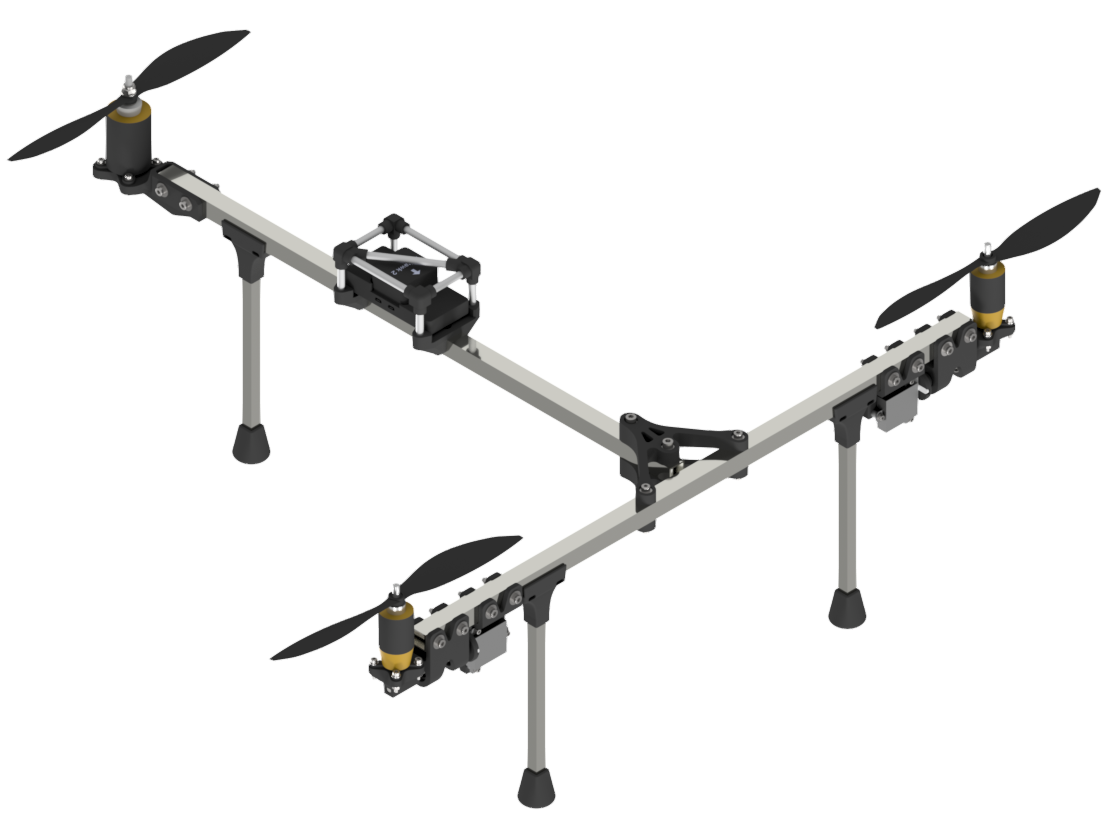
\includegraphics[width=0.9\textwidth]{Skoupa/Assembly_1_edit.png}
    \caption{Πειραματική διάταξη Τρικοπτέρου.}\label{fig:sk_assembly}
\end{figure}

Ο απλούστερος τρόπος για να δημιουργηθεί ένα τρίκόπτερο είναι η σύνδεση δύο
ράβδων σε διάταξη \tl{"}Τ\tl{"}. Στο παρακάτω σχήμα (\ref{fig:sk_frame}), 
παρουσιάζεται το βασικό πλαίσιο σε ανάπτυγμα. Οι δύο ράβδοι συνδέονται μεταξύ 
τους με τη βοήθεια των πολυμερών τεμαχίων (μαύρο χρώμα) με χρήση κοχλιών 
σύσφιξης. Τα κυλινδρικά τεμάχια, που απεικονίζονται στο σχήμα, τοποθετήθηκαν για 
να αποτρέπουν την πλαστική παραμόρφωση των αλουμινένιων ράβδων κατά τη σύσφιξη 
των κοχλιοσυνδέσεων.

\begin{figure}[H]
    \centering
    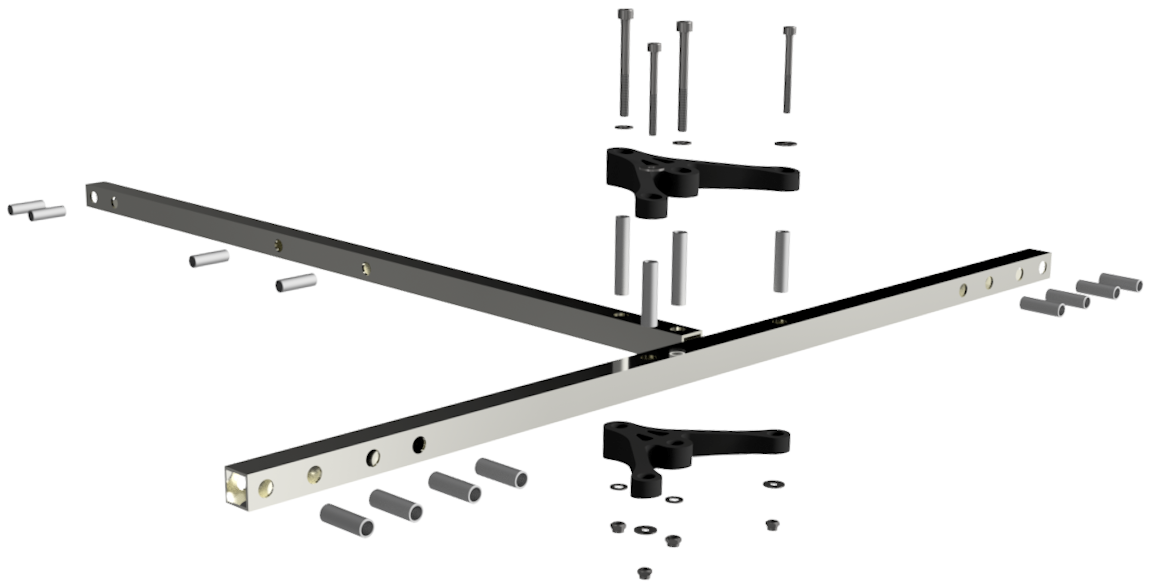
\includegraphics[width=0.8\textwidth]{Skoupa/Expl_Frame_3_edit.png}
    \caption{Πλαίσιο Τρικοπτέρου.}\label{fig:sk_frame}
\end{figure}

Κρισιμότερο στοιχείο του τρικοπτέρου αποτελεί ο μηχανισμός του
κεκλιμένου στροφείου, αφού επιτρέπει την περιστροφή του συστήματος
έλικα-κινητήρας μεταφέροντας τις δυνάμεις και ροπές των κινητήρων στο πλαίσιο.
Στο σχήμα (\ref{fig:sk_section_view}), παρουσιάζεται μια τομή του μηχανισμού,
Απαρτίζεται από τρία μέλη, το σερβομηχανισμό, την έδραση του άξονα περιστροφής 
και τον κινητήρα. Ο σερβομηχανισμός παράγει την απαιτούμενη ροπή για την
περιστροφή της βάσης του κινητήρα. Ο άξονας συνδέεται κινηματικά με την πλήμνη
του σερβομηχανισμού μέσω του συνδέσμου (α), με τον οποίο συνδέεται με σύνδεση 
μορφής. Η έδραση εξασφαλίζει την ομαλή περιστροφή αποτρέποντας την καταπόνηση 
του σερβομηχανισμού. Για την έδραση χρησιμοποιήθηκαν δύο ένσφαιρα έδρανα 
κυλίσεως (β) και μία εσωτερική ασφάλεια ατράκτου (γ) για την αξονική στήριξη του 
άξονα. Τέλος ο άξονας συνδέεται με τη βάση του κινητήρα με σύνδεση μορφής (δ).
Στο σχήμα (\ref{fig:sk_mech_ass}) παρουσιάζεται το ανάπτυγμα του μηχανισμού.

\begin{figure}[H]
    \centering
    \begin{tikzpicture}
        \node[anchor=south west,inner sep=0] (image) at (0,0)
        {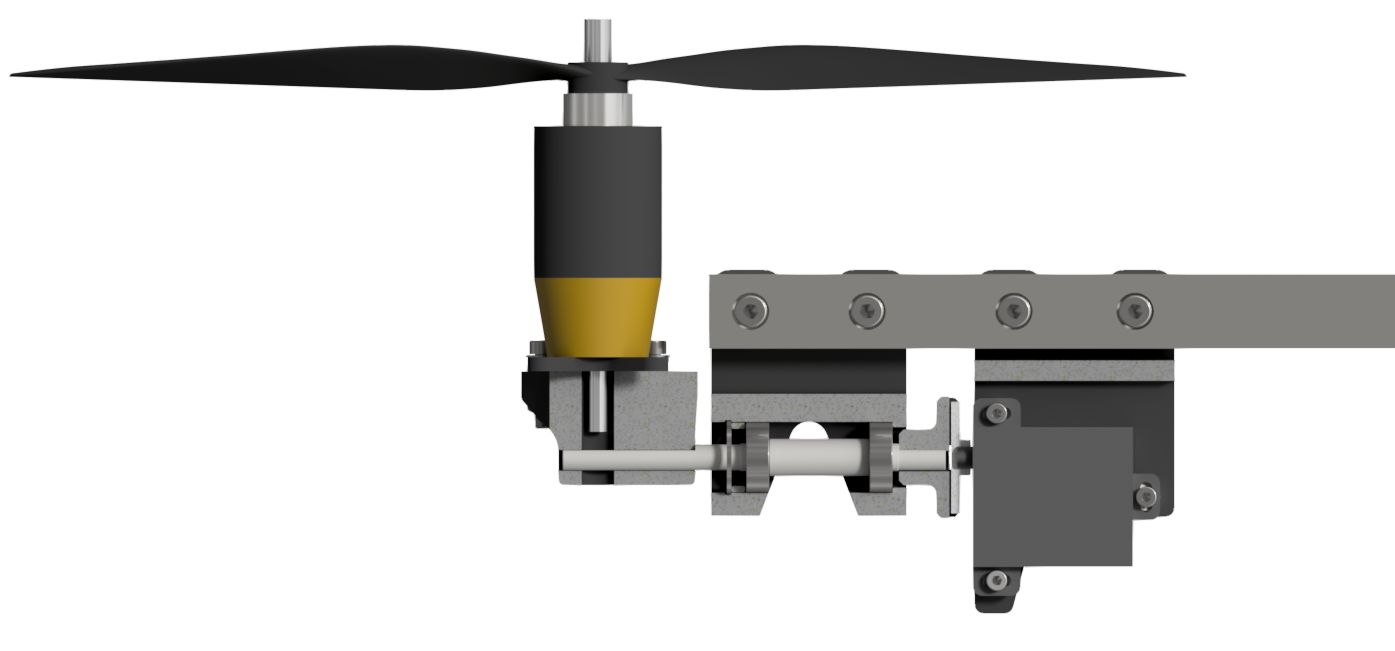
\includegraphics[width=0.8\textwidth]{Skoupa/mechanism_ray_3_edit.png}};
            \begin{scope}[x={(image.south east)},y={(image.north west)}]
                \draw (0.66, 0.26) -- (0.66, 0.15);
                \node[text width=3cm] at (0.738, 0.12) {(α)};
                \draw (0.543, 0.245) -- (0.5875, 0.15);
                \draw (0.632, 0.245) -- (0.5875, 0.15);
                \node[text width=3cm] at (0.667, 0.12) {(β)};
                \draw (0.522, 0.24) -- (0.522, 0.15);
                \node[text width=3cm] at (0.602, 0.12) {(γ)};
                \draw (0.452, 0.277) -- (0.452, 0.15);
                \node[text width=3cm] at (0.532, 0.12) {(δ)};
            \end{scope}
    \end{tikzpicture}
    \caption{Τομή Μηχανισμού Κεκλιμένου Στροφείου.}\label{fig:sk_section_view}
\end{figure}

\begin{figure}[H]
    \centering
    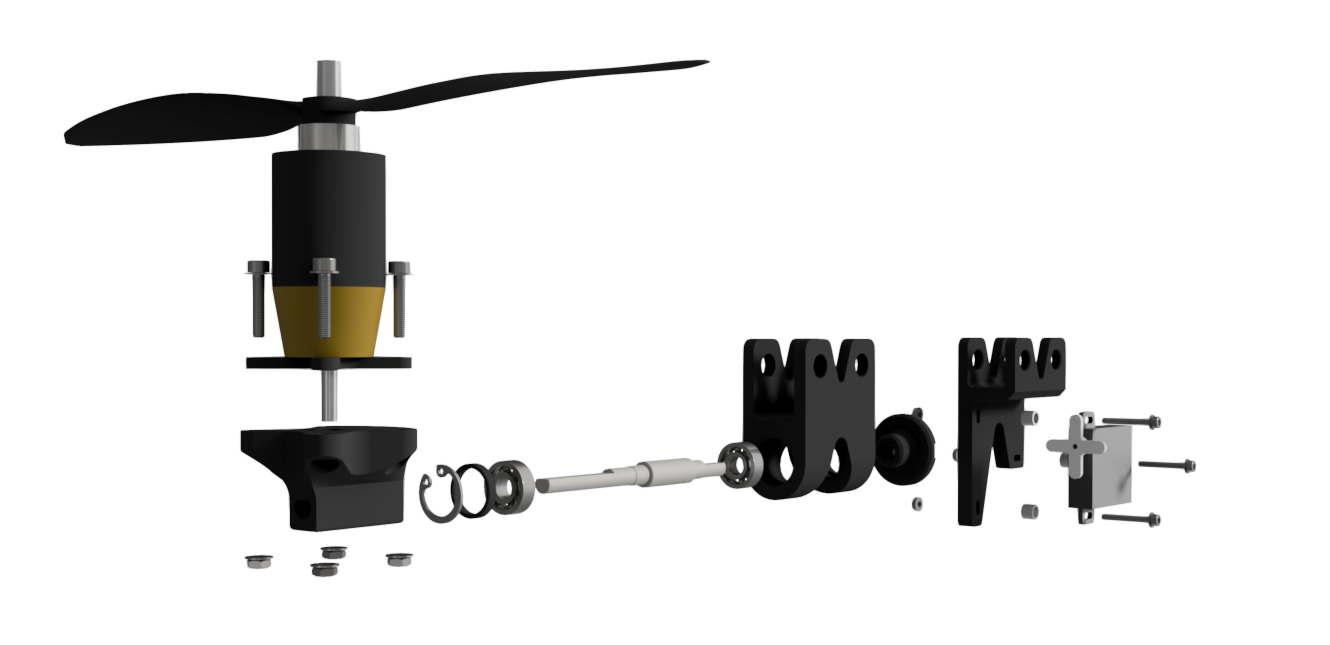
\includegraphics[width=0.8\textwidth]{Skoupa/Expl_Mechanism_edit.png}
    \caption{Ανάπτυγμα Μηχανισμού Κεκλιμένου Στροφείου.}\label{fig:sk_mech_ass}
\end{figure}

Για την στήριξη του μικροελεγκτή \tl{PixHawk}, μια βάση προσδέθηκε στο πλαίσιο 
του τρικοπτέρου. Επιπλέον, κατασκευάστηκε ένα δικτύωμα από δοκούς αλουμινίου και 
κόμβους πολυμερούς \tl{PLA} για την προστασία του από πτώσεις. Για την στήριξη 
του σταθερού οπίσθιου κινητήρα σχεδιάστηκε βάση με γνώμονα την αντοχή σε κάμψη.
Στο σχήμα παρουσιάζονται σε ανάπτυγμα τα προαναφερθέντα τεμάχια.

\begin{figure}[H]
    \begin{minipage}[t]{0.48\textwidth}
        \centering
        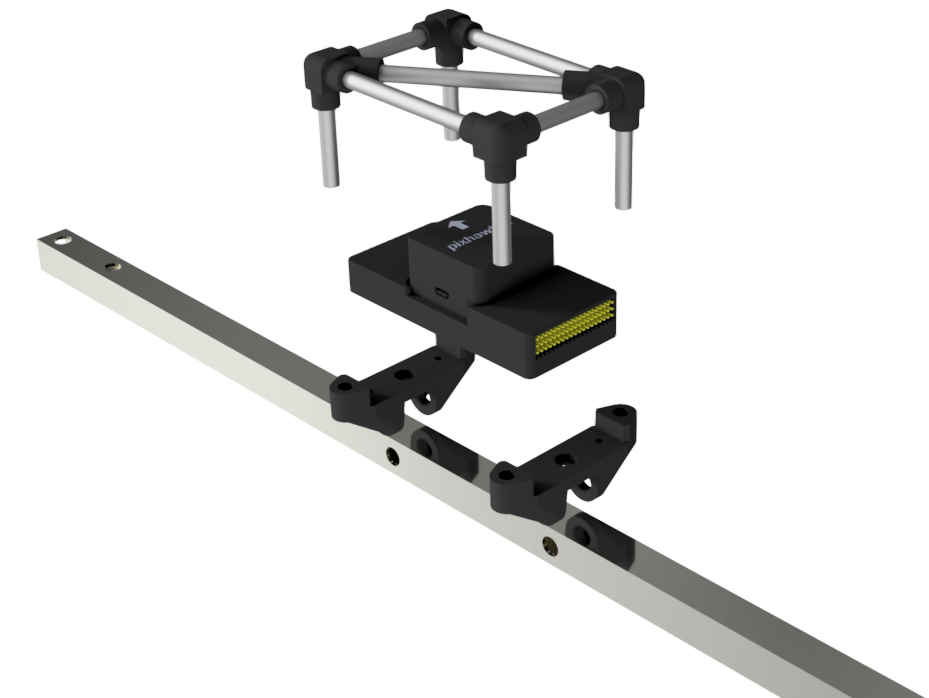
\includegraphics[width=0.8\textwidth]{Skoupa/Expl_Pixhawk_Assembly_edit.png}
        \caption*{Βάση \tl{PixHawk}}
    \end{minipage}
    \begin{minipage}[t]{0.48\textwidth}
        \centering
        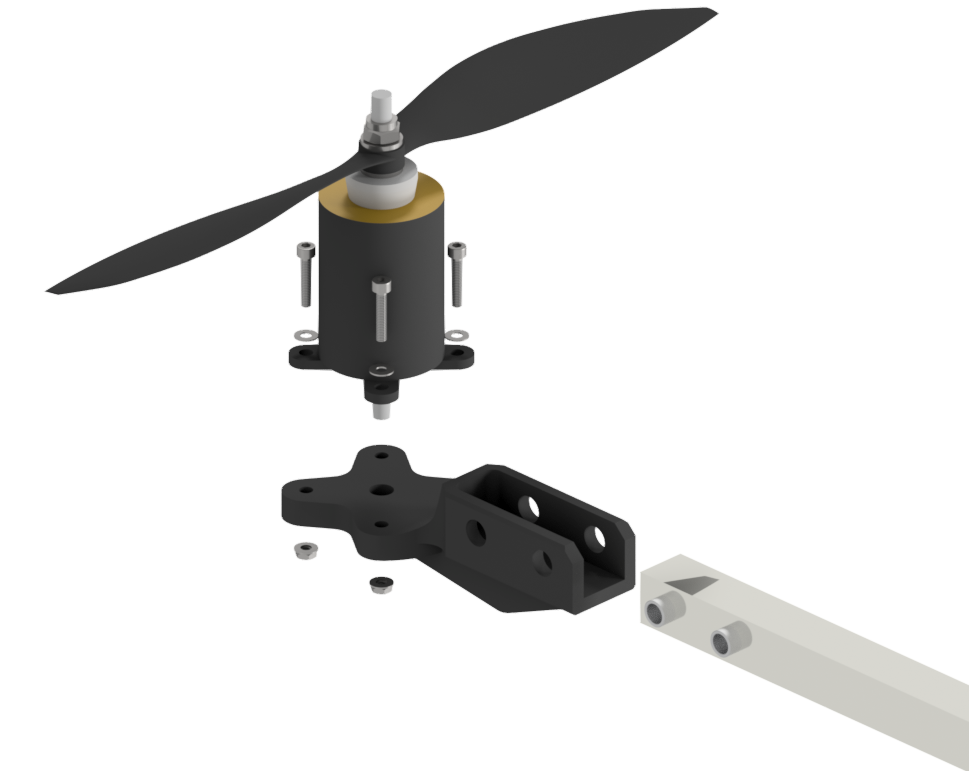
\includegraphics[width=0.8\textwidth]{Skoupa/Expl_BackMotor_edit.png}
        \caption*{Βάση Οπίσθιου Κινητήρα}
    \end{minipage}
    \caption{}\label{fig:sk_section_view}
\end{figure}

Η τελική μορφή της πειραματικής διάταξης, παρουσιάζεται στο σχήμα 
(\ref{fig:photo}).

\begin{figure}[H]
    \centering
    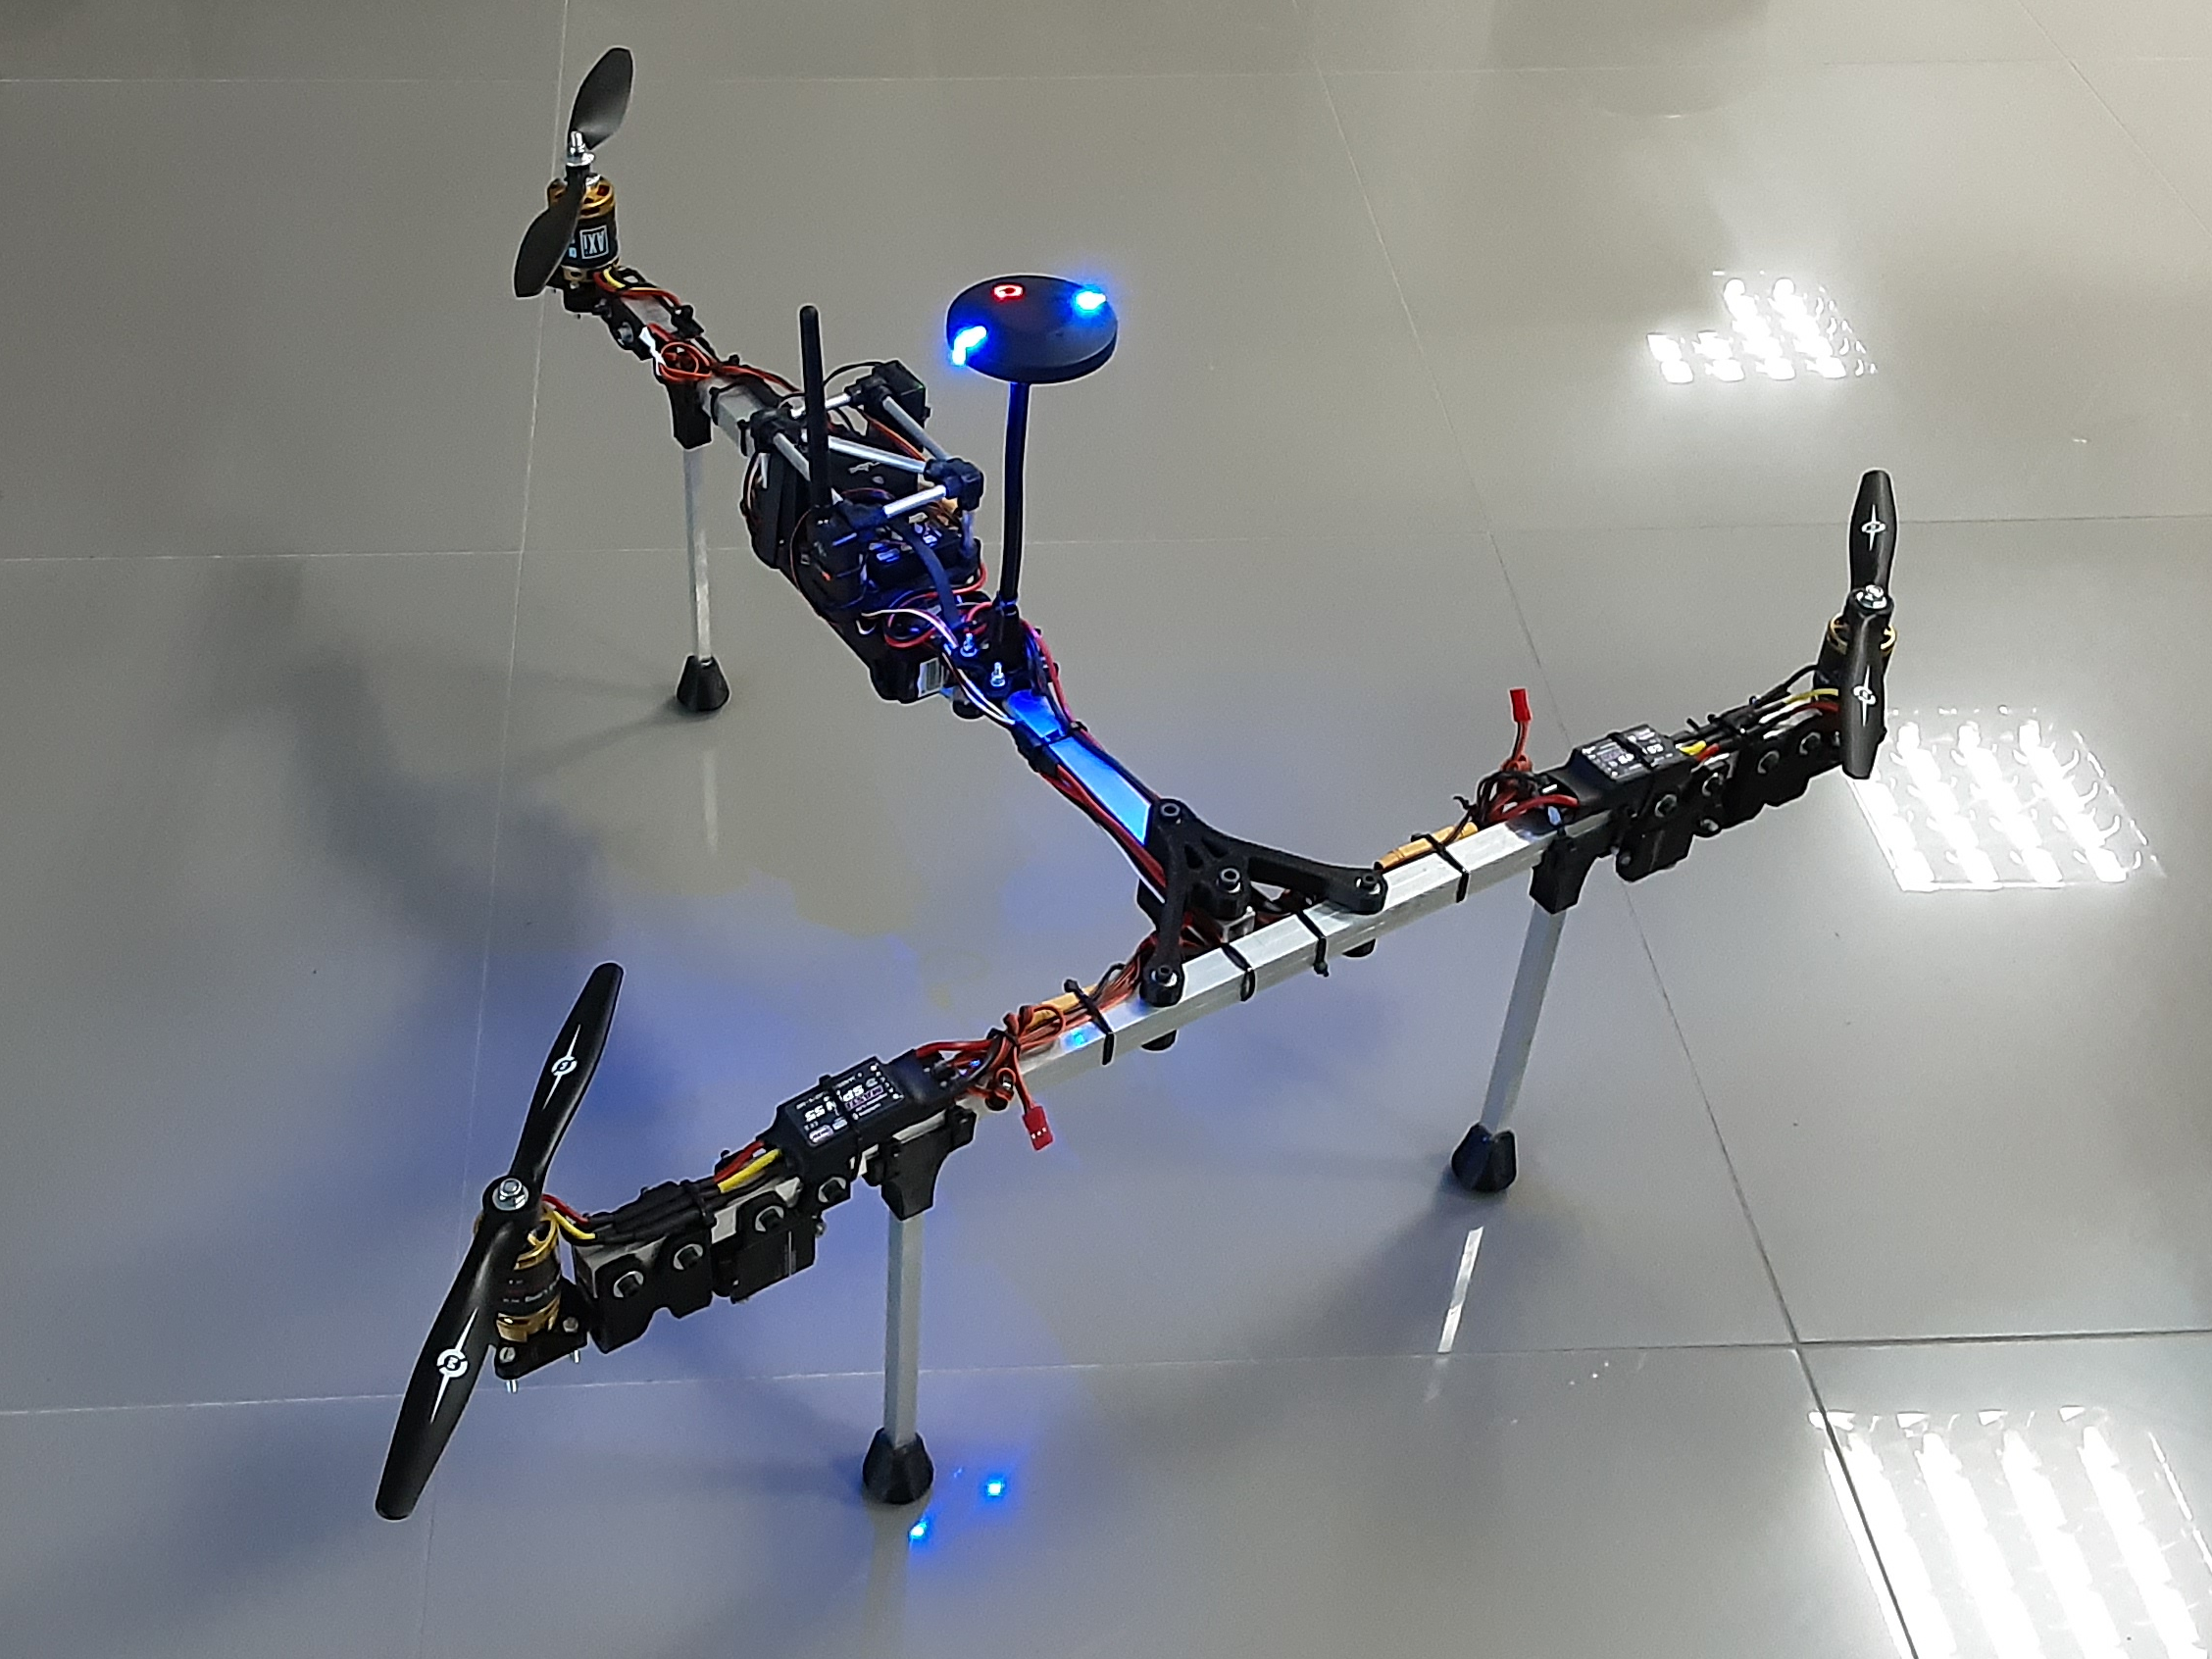
\includegraphics[width=0.8\textwidth]{Skoupa/photo.png}
    \caption{Φωτογραφία τελικής διάταξης}\label{fig:photo}
\end{figure}
 
Επιπρόσθετα, περιλαμβάνονται οι ηλεκτρονικοί ελεγκτές ταχύτητας (\tl{ESC}) των 
κινητήρων, \tl{JETI MASTERSPIN 55 PRO (2x)} και \tl{JETI MASTERSPIN 66 PRO}. Η
μπαταρία \tl{Gens ace LiPo battery 6500mAh 3s1p} και οι σερβομηχανισμοί 
\tl{Corona DS-239MG (2x)}.

\section{Ανάλυση ζεύγους Κινητήρων - Ελίκων}
\noindent Η επιλογή κινητήρων και ελίκων πραγματοποιήθηκε, με κύριο γνώμονα, 
την μέγιστη απόδοση του οχήματος \tl{MPU} κατά την πτήση του ως αερόχημα 
σταθερής πτέρυγας, η οποία αποτελεί και το μεγαλύτερο χρονικά τμήμα της πτήσης. 
Η συγκεκριμένη διαδικασία βασίζεται στην αρχή ότι η ροπή που αποδίδει ο 
κινητήρας είναι ίση με την ροπή αντίστασης της έλικας σε μόνιμη κατάσταση 
λειτουργίας. Στο σημείο αυτό, υπολογίζεται η απόδοση του κινητήρα και της έλικας
και εκτιμάται αν είναι ικανοποιητική.

Με την μοντελοποίηση του κινητήρα, έχουν ήδη περιγραφεί οι σχέσεις της ροπής με
τη γωνιακή ταχύτητα και η ανάλυση βασίζεται σε αυτές. Από τον νόμο του 
\tl{Kirchoff} (\ref{mtr:Kirchoff}), η γωνιακή ταχύτητα μπορεί να εκφρασθεί ως
\begin{equation*}
    \omega = (v - iR)K_v
\end{equation*}

Ορίζεται επιπλέον η μηχανική αποδιδόμενη ισχύς του κινητήρα ως
\begin{equation}
    P_{mech} = Q \omega = K_t(i - i_0)(v - iR)K_v = (i - i_0)(v - iR)
    \label{mtr:P_m}
\end{equation}
ενώ η προσδιδόμενη ηλεκτρική ισχύς περιγράφεται από την σχέση
\begin{equation}
    P_{elec} = vi
    \label{mtr:P_e}
\end{equation}

Από τον ορισμό της απόδοσης, η απόδοση του κινητήρα είναι το κλάσμα της ισχύς 
εξόδου του κινητήρα προς την ισχύ εισόδου.

\begin{equation}
    \eta_{m} = \frac{P_{mech}}{P_{elec}} = \left(1 - \frac{i_0}{i} \right) 
    \left(1 - \frac{iR}{v} \right)
    \label{mtr:h}
\end{equation}

Έπειτα, λύνοντας ως προς την ένταση του ρεύματος τον νόμο του \tl{Kirchoff}, 
εξάγεται η σχέση 

\begin{equation}
    i = \left( v - \frac{\omega}{K_v} \right) \frac{1}{R}.
    \label{mtr:i}
\end{equation}

Αντικαθιστώντας, λοιπόν, την (\ref{mtr:i}) στις σχέσεις (\ref{mtr:P_m}), 
(\ref{mtr:P_e}), (\ref{mtr:h}) η απόδοση, η ροπή και η αποδιδόμενη ισχύς του 
κινητήρα εκφράζονται από σχέσεις που εξαρτώνται από την τάση εισόδου και την 
γωνιακή ταχύτητα περιστροφής.
\begin{gather*}
    Q(\omega, v) = K_t \left[ \left( v - \frac{\omega}{K_v} \right) \frac{1}{R} 
    - i_0 \right]\\
    P_{mech}(\omega, v) = \left[ \left( v - \frac{\omega}{K_v} \right) 
    \frac{1}{R} - i_0 \right] \frac{\omega}{K_v}\\
    \eta_{m}(\omega, v) = \left[ 1 - \frac{i_0 R}{v - \omega/K_v} \right] 
    \frac{\omega}{vK_v}.
\end{gather*}

Οι παραπάνω εξισώσεις παράγουν τα διαγράμματα (\ref{fig_Nw}), (\ref{fig_Pmw}), 
(\ref{fig_nmw}), για τρεις διαφορετικές τιμές τάσης εισόδου

\begin{figure}[hbt!]
    \begin{minipage}[b]{0.48\linewidth}
        \centering
        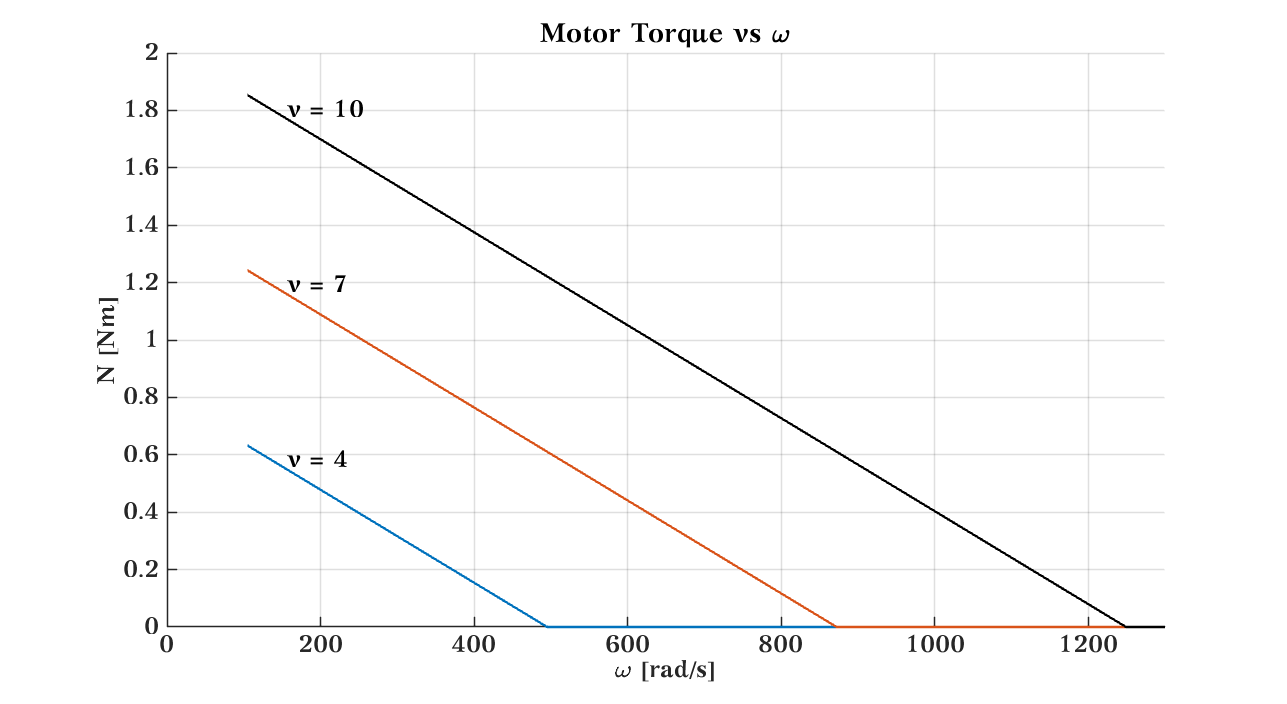
\includegraphics[width=\textwidth]{Motor/fig_N_omega.png}
        \caption{Ροπή κινητήρα}
        \label{fig_Nw}
    \end{minipage}
    \quad
    \begin{minipage}[b]{0.48\linewidth}
        \centering
        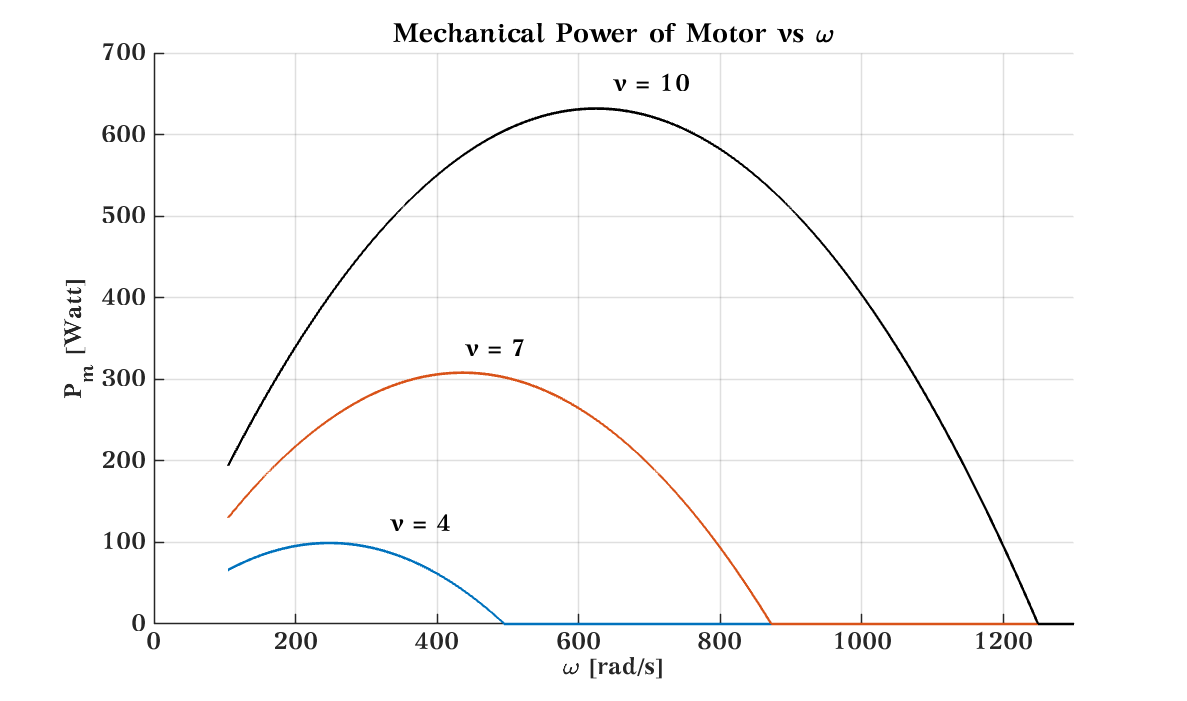
\includegraphics[width=\textwidth]{Motor/fig_Pm_omega.png}
        \caption{Μηχανική Ισχύς κινητήρα}
        \label{fig_Pmw}
    \end{minipage}
\end{figure}
\begin{figure}[H]
    \centering
    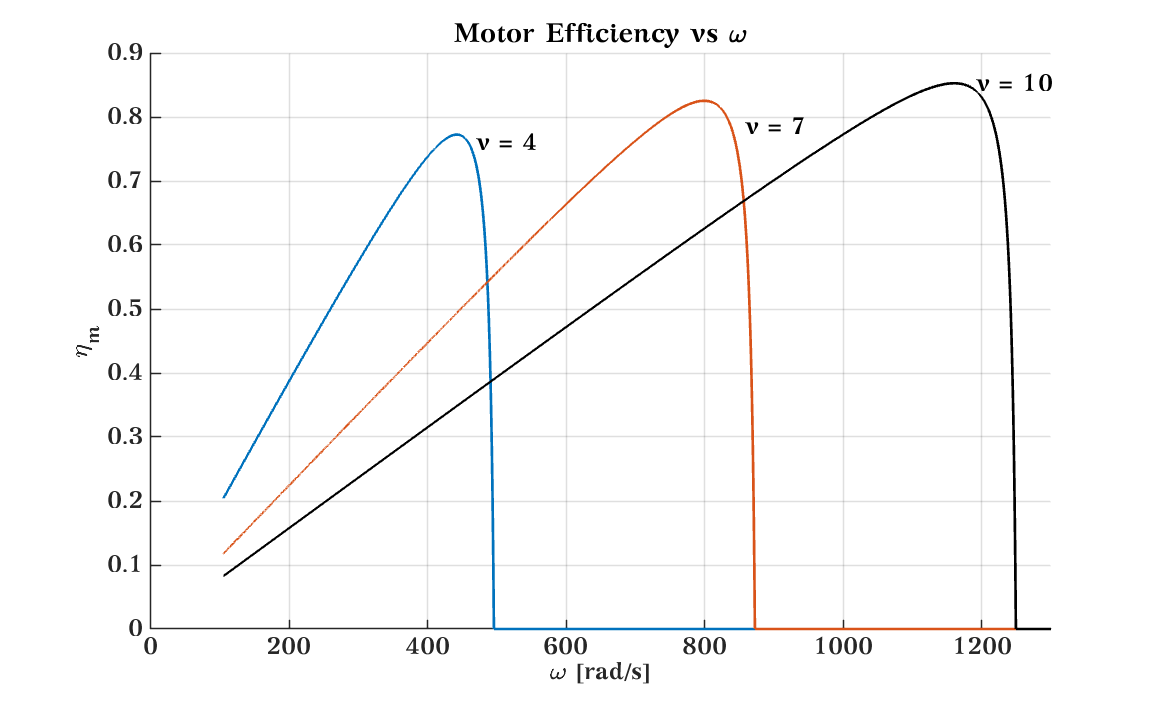
\includegraphics[scale=0.3]{Motor/fig_nm_omega.png}
    \caption{Απόδοση κινητήρα}
    \label{fig_nmw}
\end{figure}

Όσον αναφορά την δύναμη πρόωσης και την ροπή αντίστασης της έλικας,  
χρησιμοποιούνται οι σχέσεις που εξήχθησαν στην μοντελοποίηση των ελικών. Για τη 
μηχανική απόδοση της έλικας ακολουθείται ο ορισμός που χρησιμοποιήθηκε για την 
απόδοση του κινητήρα. Έτσι, η απόδοση είναι το κλάσμα της ισχύς εξόδου της 
έλικας προς την μηχανική ισχύ που παραλαμβάνει από τον κινητήρα και εκφράζεται 
ως

\begin{equation*}
    \eta_{p} = \frac{T V}{N \omega} = \frac{C_T}{2 \pi C_N}J.
\end{equation*}

Οι σχέσεις των δυνάμεων με τη μηχανική απόδοση της έλικας παράγουν τα 
διαγράμματα (\ref{fig_Mw}), (\ref{fig_Tw}), (\ref{fig_npw}), για τρεις 
διαφορετικές τιμές ταχύτητας πτήσης.

\begin{figure}[H]
    \begin{minipage}[b]{0.48\linewidth}
        \centering
        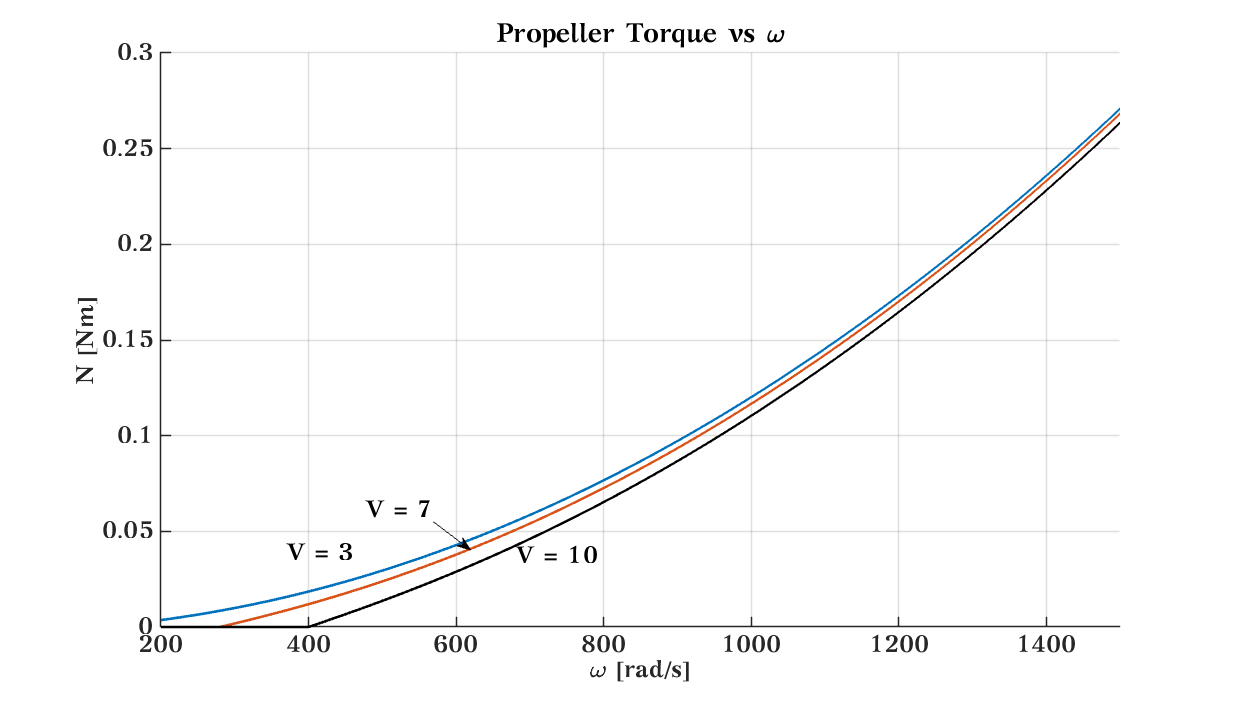
\includegraphics[width=\textwidth]{Motor/fig_M_omega.png}
        \caption{Ροπή έλικας}
        \label{fig_Mw}
    \end{minipage}
    \quad
    \begin{minipage}[b]{0.48\linewidth}
        \centering
        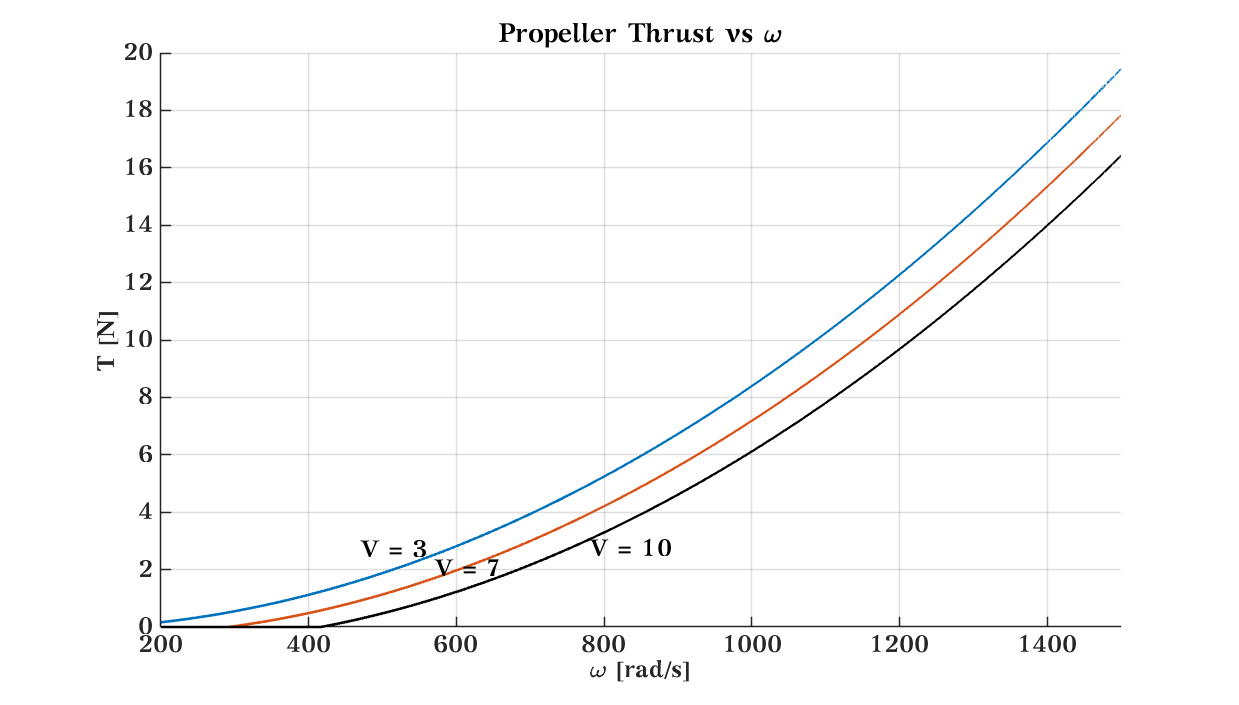
\includegraphics[width=\textwidth]{Motor/fig_T_omega.png}
        \caption{Δύναμη Ώθησης}
        \label{fig_Tw}
    \end{minipage}
\end{figure}
\begin{figure}[H]
    \centering
    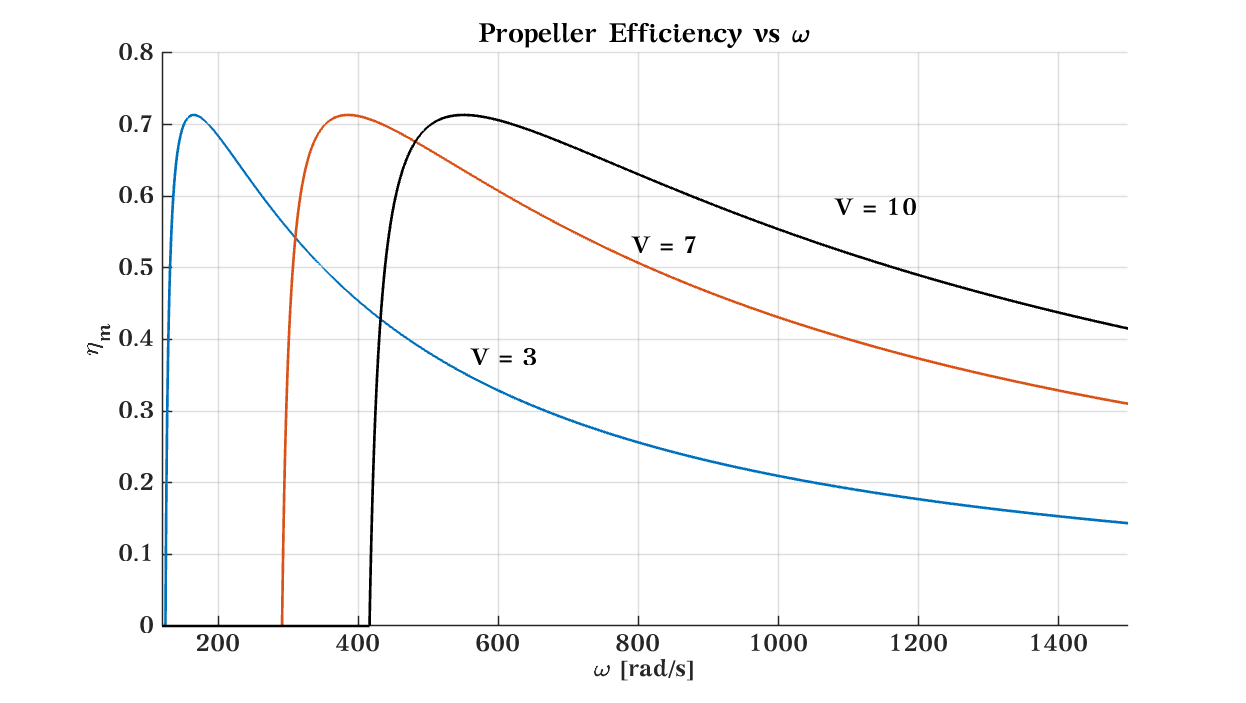
\includegraphics[scale=0.25]{Motor/fig_np_omega.png}
    \caption{Απόδοση έλικας}
    \label{fig_npw}
\end{figure}

Με τις παραπάνω πληροφορίες, γίνεται δυνατή η ανάλυση του ζεύγους κινητήρα
έλικας. Συγκεκριμένα, για κατάσταση πτήσης με παράμετρο την επιθυμητή δύναμη
πρόωσης και την επιθυμητή ταχύτητα πτήσης, βρίσκεται η ταχύτητα περιστροφής 
ισορροπίας, όπου η ροπή αντίστασης της έλικας είναι ίση με την ροπή του κινητήρα
\(Q = N\). Έχοντας βρει το συγκεκριμένο σημείο, εκτιμάται η απόδοση του κινητήρα
και της έλικας.

Η ανάλυση, όπως προαναφέρθηκε, γίνεται για πτήση του αεροχήματος ως σταθερή
πτέρυγα για μία μέση κατάσταση λειτουργίας με ταχύτητα πτήσης 
$V = 60\,km/h (= 16.67\,m/s)$ και με αεροδυναμική οπισθέλκουσα $Drag = 2.5\,N$. 
Για λειτουργία μόνιμης κατάστασης, η δύναμη πρόωσης των δύο εμπρόσθιων ελίκων 
πρέπει να ισούται με την αεροδυναμική αντίσταση. Έτσι, απαιτείται δύναμη πρόωσης 
από κάθε έλικα $T = 1.25\,N$. Στο διάγραμμα (\ref{fig_untl}) παρουσιάζονται τα 
αποτελέσματα.
\begin{figure}[H]
    \centering
    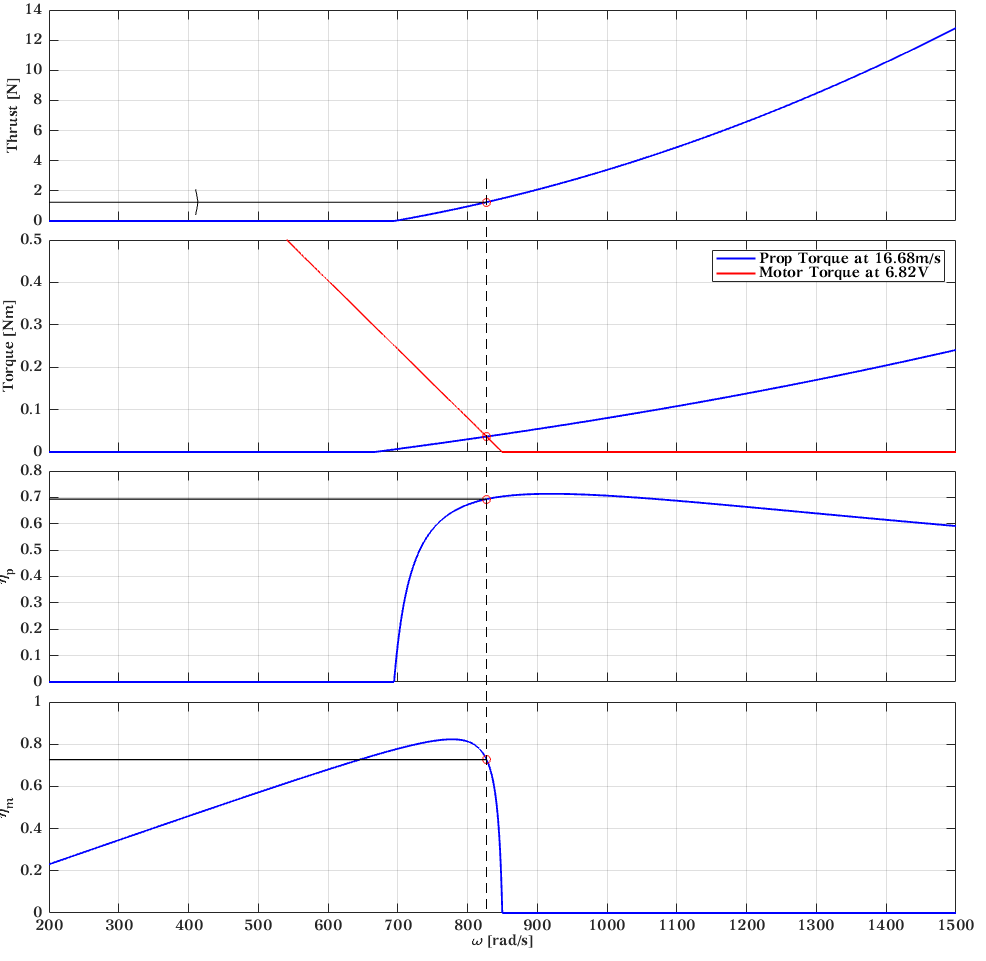
\includegraphics[scale=0.6]{Motor/untitled.png}
    \caption{Διαδικασία εύρεσης αποδόσεων και ταχύτητας περιστροφής}
    \label{fig_untl}
\end{figure}

Από την παραπάνω διαδικασία εκτιμάται η απόδοση της έλικας είναι \(\eta_{p} = 
69.33\%\) και η απόδοση του κινητήρα είναι \(\eta_{m} = 72.67\%\), ενώ η 
ταχύτητα περιστροφής της έλικας είναι \(\omega = 827.2rad/s\) και η τάση εισόδου
που απαιτείται είναι \(v = 6.82\,Volt\).

Οι δύο αποδόσεις είναι ικανοποιητικές, εφόσον η μέγιστη απόδοση του κινητήρα 
σύμφωνα με τον κατασκευαστή είναι \(\eta_{m,max} = 82\%\) ενώ από γενική θεωρία,
οι έλικες δεν μπορούν να ξεπεράσουν τα \(\eta_{p,max} = 80\%\).

Τέλος, είναι απαραίτητο να εκτιμηθούν τα φυσικά όρια λειτουργίας των 
ενεργοποιητών. Η ισχύς που απαιτεί μία έλικα για την παραγωγή δεδομένης ώθησης, 
πρέπει να καλύπτεται από τη διαθέσιμη ισχύ του κινητήρα. Εκεί, λαμβάνονται 
υπόψιν οι μέγιστες επιτρεπόμενες εντάσεις ρεύματος. Σύμφωνα με την συγκεκριμένη
διαδικασία προκύπτουν $\omega_{b,max} = 11000\,rpm$, $\omega_{l,r,max} = 13000\,
rpm$.